% ECHO, DASFAA 2027 research track submission (LNCS, double-blind, 16 pages).
\documentclass[runningheads]{llncs}
\usepackage[T1]{fontenc}
\usepackage{amsmath,amssymb}
\usepackage{booktabs,multirow,array}
\usepackage{graphicx}
\usepackage{xcolor}
\usepackage{wrapfig}
\usepackage[hidelinks]{hyperref}
\renewcommand\UrlFont{\color{blue}\rmfamily}

\emergencystretch=1em
\renewcommand{\topfraction}{0.9}
\renewcommand{\bottomfraction}{0.8}
\renewcommand{\textfraction}{0.08}
\renewcommand{\floatpagefraction}{0.85}

\newcommand{\model}{ECHO}
\newcommand{\hone}{H@1}
\newcommand{\hten}{H@10}
\newcommand{\lam}{\lambda}
\newcommand{\spm}{\ensuremath{\scriptstyle\,\pm\,}}
\newcommand{\para}[1]{\smallskip\noindent\textbf{#1}}

\begin{document}

\title{Dyadic Event Streams as Evidence for Temporal Knowledge Graph Forecasting}
\titlerunning{Dyadic Event Streams for TKG Forecasting}

\author{Anonymous Author(s)}
\authorrunning{Anonymous Author(s)}
\institute{Anonymous Institution(s)}

\maketitle

\begin{abstract}
Temporal knowledge graph (TKG) forecasting predicts the missing object of a query $(s, r, ?, t)$ from the facts observed before $t$. Most strong models rely on the history of the query pair $(s, r)$, either through a copy mechanism or through a graph built from that history. We find that this view leaves out a large part of the available evidence. On ICEWS18, 23.4\% of the test queries have an answer that never appeared with $(s, r)$ but did interact with the subject under another relation, and copy-based scoring cannot rank such answers at all. We therefore take the \emph{dyad}, i.e., the entity pair $(s, o)$ together with all typed and timestamped events between the two entities, as the basic unit of evidence, and propose \model{}. \model{} adds four intensities: a structural intensity from snapshot evolution, a popularity intensity, a dyadic intensity that encodes the event stream of each dyad with a small Transformer, and a path intensity that propagates dyadic states along the recent edges of each candidate. Experiments on five benchmarks show that \model{} obtains the best MRR and Hits@1 on YAGO, WIKI and GDELT among the compared methods and competitive results on ICEWS. A stratified evaluation further shows where each component contributes.

\keywords{Temporal knowledge graph \and Link forecasting \and Event streams \and Point process \and Stratified evaluation}
\end{abstract}

% ─────────────────────────────────────────────────────────────────────────
\section{Introduction}
\label{sec:intro}

A temporal knowledge graph (TKG) stores facts as quadruples $(s, r, o, t)$, where a subject $s$ and an object $o$ are connected by a relation $r$ at time $t$. TKG forecasting, also called extrapolation, asks for the object of a query $(s, r, ?, t)$ given only the facts before $t$. It supports applications such as event prediction, crisis early warning and the maintenance of evolving knowledge bases, and it is usually evaluated on political event data (ICEWS, GDELT) and on yearly encyclopedic graphs (YAGO, WIKI). Existing methods fall into several groups: snapshot-based evolution models~\cite{jin2020renet,li2021regcn,li2022cen,dong2025dimnet}, copy mechanisms~\cite{zhu2021cygnet,xu2023cenet}, path- and rule-based reasoners~\cite{han2021xerte,sun2021titer,liu2022tlogic,dong2023daemon,dong2024tipnn}, models with global history graphs~\cite{li2022tirgn,chen2024logcl,chen2025cogntke}, and diffusion models~\cite{cai2024diffutkg}.

Several recent studies point out that repetition explains much of the performance on these benchmarks. A recurrency baseline with a few hand-set parameters, which only looks up the objects that appeared with $(s, r)$ before, is competitive with many trained models~\cite{gastinger2024history}, and more than 80\% of the ICEWS test events have occurred earlier~\cite{strikingness2026}. Consequently, the common design of current models is to read the history of the query pair $(s, r)$ as well as possible.

\begin{wrapfigure}{r}{0.50\textwidth}
  \vspace{-18pt}
  \centering
  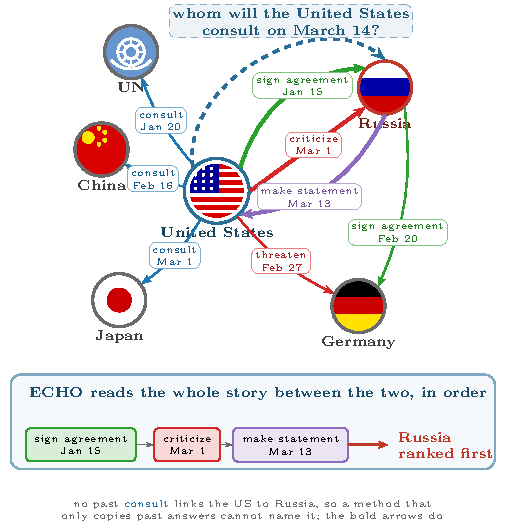
\includegraphics[width=0.49\textwidth]{figures/fig_intro.pdf}
  \caption{A toy example. The subject has never consulted the answer before, but the two have a recent history under other relations.}
  \label{fig:intro}
  \vspace{-14pt}
\end{wrapfigure}

This design has a blind spot. Consider the query in Fig.~\ref{fig:intro}, which asks whom the United States will consult. A model that copies from the history of (United States, \emph{consult}) can only propose the entities that were consulted before. The correct answer has never been consulted by the subject, yet the two entities signed an agreement, exchanged criticism and made statements within the last weeks. This information is present in the data, but it is attached to the entity pair and not to the query pair.

We call the ordered pair $(s, o)$ together with all events between the two entities, under any relation and in either direction, a \emph{dyad}. Before designing a model we measure how much evidence the dyad carries (Sect.~\ref{sec:diag}). On ICEWS18, 50.6\% of the test queries have an answer that already occurred with $(s, r)$; 23.4\% have an answer that never occurred with $(s, r)$ but interacted with $s$ under another relation; and for 26.0\% the answer never interacted with $s$. The second group is not reachable by any copy mechanism. Moreover, a simple counter over dyad events, with no trained parameters except relation co-occurrence statistics, raises the MRR of a recurrence counter on ICEWS18 from 28.0 to 31.8, which is close to the reported result of DaeMon~\cite{dong2023daemon}. On YAGO and WIKI the second group is almost empty (0.1\%), so the benefit of the dyad is expected mainly on event data.

Based on these observations we propose \model{}. It models the answer of a query as the outcome of a superposition of four point processes whose intensities are added. The central one is a \emph{dyadic intensity}: for each candidate, the most recent events of the dyad are turned into tokens of relation type and elapsed time and encoded by a two-layer Transformer, so that repetition, the influence of other relations, reciprocity and event order are handled by the same module. A \emph{path intensity} extends the dyad by one hop and reaches answers that are partners of the subject's partners. A \emph{popularity intensity} and a \emph{structural intensity} from snapshot evolution cover all entities. In addition, the candidates of a query attend to each other before scoring.

Our contributions are summarized as follows:
\begin{enumerate}
  \item We introduce a data-only analysis that splits test queries into recurrent, dyad-only and cold strata, and show that the dyad-only stratum accounts for about a quarter of the ICEWS queries and cannot be handled by copy mechanisms.
  \item We propose \model{}, which adds four intensities and encodes the typed and timed event stream of each dyad with a Transformer, together with a path intensity and attention across the candidates of a query.
  \item We conduct experiments on five benchmarks with three seeds. \model{} achieves the best MRR and \hone{} on YAGO, WIKI and GDELT among the compared methods and competitive results on ICEWS18 and ICEWS14s.
  \item We provide a stratified evaluation and ablation study, which show that each component contributes on the stratum it is designed for, and which also identify the queries where the model remains weak.
\end{enumerate}

% ─────────────────────────────────────────────────────────────────────────
\section{Related Work}
\label{sec:related}

\para{Copy and recurrence.} CyGNet~\cite{zhu2021cygnet} combines a copy mode over the objects that appeared with $(s, r)$ and a generation mode over all entities. CENET~\cite{xu2023cenet} learns to separate historical from non-historical queries with contrastive learning. TiRGN~\cite{li2022tirgn} adds a global history encoder to a local recurrent encoder. Gastinger et al.~\cite{gastinger2024history} show that a non-parametric recurrency baseline is competitive with many learned models, and CountTRuCoLa~\cite{gastinger2026counttrucola} extends this idea to rules that combine recency and frequency. In all of these works, the history is defined with respect to the query pair $(s, r)$.

\para{Snapshot evolution.} RE-NET~\cite{jin2020renet} and RE-GCN~\cite{li2021regcn} apply a relational GCN to each snapshot and a recurrent unit across snapshots. CEN~\cite{li2022cen} handles evolution patterns of different lengths, HiSMatch~\cite{li2022hismatch} matches the historical structures of queries and candidates, and DiMNet~\cite{dong2025dimnet} disentangles active and stable features with multi-span evolution. The structural intensity of \model{} follows this line.

\para{Global history, paths and rules.} LogCL~\cite{chen2024logcl} builds a query-related global graph and aligns it with the local view by contrastive learning, and CognTKE~\cite{chen2025cogntke} combines one-hop and multi-hop reasoning. xERTE~\cite{han2021xerte} and TITer~\cite{sun2021titer} search a query-centered subgraph, DaeMon~\cite{dong2023daemon} and TiPNN~\cite{dong2024tipnn} model temporal paths between the subject and the candidates, and TLogic~\cite{liu2022tlogic} mines temporal logical rules. Compared with these methods, \model{} represents the history between the subject and a candidate as an ordered event sequence instead of a graph or a set of rules.

\para{Point processes and diffusion.} Know-Evolve~\cite{trivedi2017knowevolve} and GHNN~\cite{han2020ghnn} model facts with temporal point processes. GHNN notes that assigning a separate process to every possible link is infeasible because of the number of event types. In \model{}, a dyad is instantiated only if it has history, which keeps the number of sequences per query small. DiffuTKG~\cite{cai2024diffutkg} formulates forecasting as a conditional denoising process.

\para{Evaluation.} Gastinger et al.~\cite{gastinger2023apples} report that differences in filtering, dataset versions and prediction settings change results by several points. Other studies observe that aggregate metrics are dominated by repeated facts~\cite{gastinger2024history,zhang2026evolution,strikingness2026}. This motivates the stratified evaluation used in this paper.

% ─────────────────────────────────────────────────────────────────────────
\section{Preliminaries}
\label{sec:prelim}

\para{Task.} A TKG is a set of quadruples $\mathcal{G} = \{(s, r, o, t)\}$ over entities $\mathcal{E}$ with $|\mathcal{E}| = N$, relations $\mathcal{R}$ and discrete timestamps. One time step corresponds to one snapshot (a day on ICEWS, fifteen minutes on GDELT, a year on YAGO and WIKI). As in previous work, each fact is also added in its inverse form $(o, r^{-1}, s, t)$, so that there are $2|\mathcal{R}|$ relation types and only object queries $(s, r, ?, t)$ need to be answered. The model ranks all entities using facts with timestamps smaller than $t$. At test time the ground-truth history before $t$ is available, as in RE-GCN~\cite{li2021regcn}.

\para{Dyad stream.} For a query $(s, r, ?, t)$ and a candidate $o$, the dyad stream $\mathcal{D}_{so}(t)$ is the time-ordered sequence of all events $(\rho, \tau)$ with $\tau < t$ and $(s, \rho, o, \tau) \in \mathcal{G}$. Since inverse facts are included, events in which $o$ acted on $s$ appear with the inverse relation type. The triple history of $o$ is the part of the stream with $\rho = r$.

\begin{definition}[Strata]
\label{def:strata}
A test query with answer $o^\star$ is \emph{recurrent} if $o^\star$ has a non-empty triple history, \emph{dyad-only} if it is not recurrent but $\mathcal{D}_{so^\star}(t)$ is non-empty, and \emph{cold} otherwise. A recurrent query is \emph{blocked} if another object with triple history is at least as recent and at least as frequent as $o^\star$, and \emph{clean} otherwise. A cold query is \emph{cold-2hop} if $o^\star$ is a neighbor of a recent partner of $s$, and \emph{cold-far} otherwise.
\end{definition}

The strata depend only on the data. A scoring function of the form $f(\mathrm{count}) \cdot g(\Delta t)$ with non-decreasing $f$ and non-increasing $g$, which covers the usual copy scores, cannot rank the answer of a blocked query first, and it has no input for a dyad-only query.

% ─────────────────────────────────────────────────────────────────────────
\section{Motivating Analysis}
\label{sec:diag}

We first examine the data without training a model. Two questions are considered: how large the strata are, and whether the dyad provides useful ranking information.

\begin{figure}[t]
  \centering
  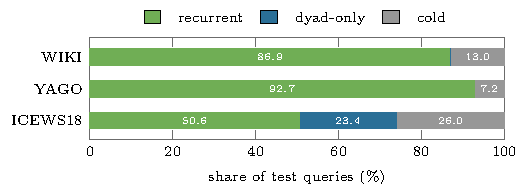
\includegraphics[width=0.66\textwidth]{figures/fig_strata.pdf}
  \caption{Share of test queries in each stratum. The dyad-only stratum is large on the ICEWS datasets and nearly empty on YAGO and WIKI.}
  \label{fig:strata}
\end{figure}

\para{Size of the strata.} Fig.~\ref{fig:strata} shows the proportions. On both ICEWS datasets about half of the queries are recurrent, and the dyad-only and cold strata each take about a quarter. On YAGO and WIKI most facts last for years, so the dyad-only stratum is only 0.1\%. We therefore expect a model that reads the dyad to gain on ICEWS but not on YAGO and WIKI. This expectation is examined in Sect.~\ref{sec:ablation}.

\para{Untrained counters.} We compare simple counters that share the time decay $w(\Delta) = e^{-0.3\Delta} + 0.2\,e^{-0.02\Delta} + 0.02$ and use only events before the query time. \emph{Recurrence} sums $w$ over past $(s, r, o)$ events. \emph{Blind dyad} sums $w$ over all past events between $s$ and $o$. \emph{Typed dyad} additionally weights each event of type $\rho$ by the frequency, counted on the training set, with which a $\rho$ event on a dyad is followed by an $r$ event within seven steps. \emph{Popularity} sums $w$ over past $(\cdot, r, o)$ events. \emph{Backoff} ranks by recurrence, then typed dyad, then popularity.

\begin{table}[t]
  \centering
  \caption{Results of untrained counters (time-aware filtered, in \%). ICEWS18 is evaluated on 30,000 sampled test queries and ICEWS14s on all test queries.}
  \label{tab:diag}
  \setlength{\tabcolsep}{6pt}
  \begin{tabular}{l ccc ccc}
    \toprule
    & \multicolumn{3}{c}{ICEWS18} & \multicolumn{3}{c}{ICEWS14s} \\
    \cmidrule(lr){2-4}\cmidrule(lr){5-7}
    Counter & MRR & \hone{} & \hten{} & MRR & \hone{} & \hten{} \\
    \midrule
    Recurrence & 28.02 & 20.93 & 41.41 & 37.08 & 30.80 & 48.50 \\
    Blind dyad & 24.55 & 14.71 & 45.10 & 36.78 & 26.43 & 57.31 \\
    Typed dyad & 30.65 & 21.05 & 49.82 & 42.72 & 33.73 & 60.39 \\
    Popularity & 12.09 &  6.64 & 23.13 & 15.50 &  8.21 & 30.19 \\
    Backoff    & \textbf{31.82} & \textbf{22.55} & \textbf{49.88} & \textbf{43.26} & \textbf{34.08} & \textbf{60.85} \\
    \bottomrule
  \end{tabular}
\end{table}

Table~\ref{tab:diag} lists the results. Using the dyad instead of the triple history improves MRR from 28.0 to 31.8 on ICEWS18 and from 37.1 to 43.3 on ICEWS14s. For reference, the reported MRR of DaeMon on ICEWS18 is 31.85~\cite{dong2025dimnet} and that of TLogic on ICEWS14 is 43.04~\cite{liu2022tlogic}. On the dyad-only stratum, where recurrence scores zero, the blind dyad counter reaches 42.3 \hten{} on ICEWS18.

Two limitations of the counters guide the model design. First, on the dyad-only stratum the typed counter is not better than the blind one (20.33 vs.\ 20.01 MRR on ICEWS18), which suggests that a fixed confidence per relation pair is too weak to use relation types and that a sequence model is needed. Second, none of the counters reaches the cold stratum. However, 54\% of the cold answers on ICEWS18 are neighbors of one of the 96 most recent partners of the subject. This motivates the path intensity in Sect.~\ref{sec:path}.

% ─────────────────────────────────────────────────────────────────────────
\section{Method}
\label{sec:method}

\begin{figure}[t]
  \centering
  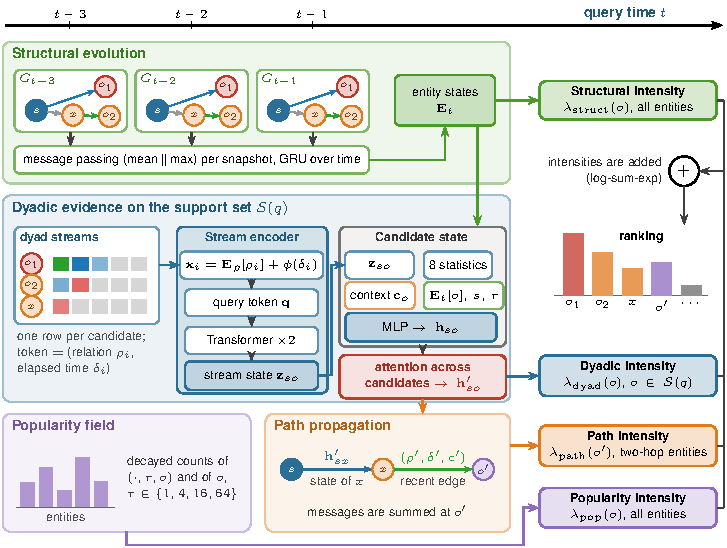
\includegraphics[width=\textwidth]{figures/fig_framework.pdf}
  \caption{Overview of \model{}. Entity states are evolved over recent snapshots (top). For each candidate in the support set, the event stream between the subject and the candidate is encoded by a Transformer and combined with summary statistics, the candidate's context and the entity and query vectors; the candidates of a query then attend to each other (middle). The refined candidate states are also propagated along the candidates' recent edges, and a popularity field scores all entities (bottom). The four intensities are added and the entities are ranked (right).}
  \label{fig:overview}
\end{figure}

Fig.~\ref{fig:overview} gives an overview of \model{}. For a query $q = (s, r, ?, t)$, the model computes four log-intensities for the candidate objects and combines them.

\subsection{Superposition of Intensities}

We regard the object of a query as the mark of the first event of a superposition of marked point processes. Since the intensity of a superposition is the sum of the component intensities, the score of an object is
\begin{equation}
  \log \lam(o \mid q) = \log\big(\lam_{\mathrm{struct}}(o \mid q) + \lam_{\mathrm{pop}}(o \mid q) + \lam_{\mathrm{dyad}}(o \mid q) + \lam_{\mathrm{path}}(o \mid q)\big),
  \label{eq:super}
\end{equation}
which is computed from the four log-intensities with the log-sum-exp operation. The probability that $o$ is the answer is the normalized intensity,
\begin{equation}
  P(o \mid q) = \frac{\lam(o \mid q)}{\sum_{o' \in \mathcal{E}} \lam(o' \mid q)} .
  \label{eq:prob}
\end{equation}
The four components differ in the evidence they read and in the entities they cover. The structural and popularity intensities are defined for all $N$ entities. The dyadic intensity is defined only for entities that have interacted with the subject, and the path intensity only for entities within two hops; outside these sets the corresponding intensity is zero.

We use a sum instead of the gate or mixing weight that is common in copy-generation models~\cite{zhu2021cygnet} for two reasons. First, a component without evidence for a candidate simply adds nothing and cannot suppress the others, so no mechanism is needed to decide which component to trust for a given query. Second, the contribution of each component to a prediction can be read off directly, which we use in the stratified analysis of Sect.~\ref{sec:ablation}. The popularity, dyadic and path components each have a learnable bias initialized to $-2$, which keeps their initial contribution small.

\subsection{Support Set}

The dyadic and path intensities are computed on a support set $\mathcal{S}(q) \subset \mathcal{E}$ that is constructed from the history of the subject. It is the union of two parts: the $S_2$ objects that most recently occurred with $(s, r)$, which covers the candidates of a copy mechanism, and the $S_1$ entities that most recently interacted with $s$ under any relation and in either direction, which covers the dyad-only candidates. An entity that appears in both parts is kept once. With $S_1 = 96$ and $S_2 = 64$, only about 4\% of the ICEWS18 test queries have an answer that interacted with the subject but lies outside the support set; these belong to subjects with very many partners. All inputs of a candidate are computed from events before $t$, once per timestamp, and shared by the queries of that timestamp.

\subsection{Dyadic Intensity}

\para{Stream encoder.} For a candidate $o \in \mathcal{S}(q)$, the $L$ most recent events of $\mathcal{D}_{so}(t)$ are mapped to tokens
\begin{equation}
  \mathbf{x}_i = \mathbf{E}_\rho[\rho_i] + \phi(\delta_i), \qquad i = 1, \dots, L,
\end{equation}
where $\rho_i$ is the relation type of the $i$-th event and $\delta_i = t - \tau_i$ is its elapsed time. The time encoding is
\begin{equation}
  \phi(\delta) = \mathbf{W}_\phi \big[\tfrac{1}{4}\ell,\ \sin(\omega_1 \ell), \cos(\omega_1 \ell), \dots, \sin(\omega_8 \ell), \cos(\omega_8 \ell)\big], \quad \ell = \log(1 + \delta),
  \label{eq:time}
\end{equation}
with frequencies $\omega_k$ geometrically spaced in $[1, 24]$. Unlike an exponential decay kernel, this encoding does not force the influence of an event to decrease with time. A query token $\mathbf{q} = \mathbf{E}_q[r] + \mathbf{W}_s \mathbf{E}_t[s]$ is placed in front of the sequence, where $\mathbf{E}_t[s]$ is the evolved state of the subject (Sect.~\ref{sec:struct}). The sequence $[\mathbf{q}; \mathbf{x}_1; \dots; \mathbf{x}_L]$ is fed into two pre-norm Transformer blocks with multi-head self-attention, and the layer-normalized output at the query position is the stream state $\mathbf{z}_{so}$. Streams with fewer than $L$ events are padded, and padded positions are masked in the attention. The tokens do not depend on the query relation, so a stream is built once per (subject, candidate) pair and shared by all queries of that subject.

Placing the query relation in the sequence lets the encoder decide which past events matter for this query. Several patterns that are usually handled by separate modules are covered in this way: (i) \emph{repetition}, when earlier events have the type $\rho_i = r$; (ii) \emph{cross-relation influence}, when events of another type make $r$ more likely, e.g., a negotiation followed by an agreement; (iii) \emph{reciprocity}, since events initiated by $o$ appear in the stream with inverse types; and (iv) \emph{order}, because the sequence $\rho_1 \rho_2$ is encoded differently from $\rho_2 \rho_1$.

\para{Candidate state.} Because the stream is truncated to $L$ events, it does not preserve counts over the full history. We therefore add eight statistics
\begin{equation}
  \begin{aligned}
  \mathbf{a}_{so} = \big[&\log(1{+}n_{sro}),\ \log(1{+}\delta_{sro}),\ \log(1{+}\bar{g}_{sro}),\ \mathbf{1}[n_{sro} {>} 0],\\
  &\log(1{+}n_{so}),\ \log(1{+}\delta_{so}),\ \log(1{+}\bar{g}_{so}),\ n_{sro}/n_{so}\big],
  \end{aligned}
\end{equation}
where $n$, $\delta$ and $\bar{g}$ denote the number of events, the time since the last event and the mean gap between consecutive events, for the triple $(s, r, o)$ and for the dyad $(s, o)$, respectively. We also describe the recent activity of the candidate itself. Its $P_2$ most recent distinct edges $(\rho', o', \delta', c')$, where $\delta'$ is the time since the edge last occurred and $c'$ the number of its occurrences, are embedded as $\mathbf{E}''_{\rho'} + \phi(\delta') + \mathbf{W}_c \log(1 + c')$, transformed by a feed-forward layer and averaged into a context vector $\mathbf{c}_o$. The time encodings of the stream, the context and the path share the form of Eq.~(\ref{eq:time}) but have separate parameters. The candidate state is
\begin{equation}
  \mathbf{h}_{so} = \mathrm{MLP}\big([\mathbf{z}_{so};\ \mathrm{LN}(\mathbf{a}_{so});\ \mathbf{W}_e \mathbf{E}_t[o];\ \mathbf{c}_o;\ \mathbf{q}_s;\ \mathbf{q}_r]\big),
\end{equation}
where $\mathrm{LN}$ is layer normalization, $\mathbf{q}_s = \mathbf{W}'_s \mathbf{E}_t[s]$ and $\mathbf{q}_r = \mathbf{W}_r \mathbf{R}[r]$.

\para{Attention across candidates.} Scoring each candidate independently cannot express relative patterns, for example that the answer alternates among several partners. Therefore the states of all candidates of a query pass through one more attention block over the support set, which yields refined states $\mathbf{h}'_{so}$. The dyadic log-intensity is
\begin{equation}
  \log\lam_{\mathrm{dyad}}(o \mid q) = \mathbf{w}^\top \mathbf{h}'_{so} + b_{\mathrm{dyad}}, \qquad o \in \mathcal{S}(q),
\end{equation}
and $-\infty$ outside the support set. This block is used on the event datasets and disabled on YAGO and WIKI according to validation results (Sect.~\ref{sec:setup}).

\subsection{Path Intensity}
\label{sec:path}

The dyadic intensity cannot score an entity that has never interacted with $s$. The path intensity extends it by one hop. Each candidate $x \in \mathcal{S}(q)$ sends its state along its $P_2$ most recent edges $(x, \rho', o', \delta', c')$:
\begin{equation}
  \mathbf{m}_{x \to o'} = (\mathbf{W}_u \mathbf{h}'_{sx}) \odot \mathrm{MLP}\big(\mathbf{E}'_{\rho'} + \phi(\delta') + \mathbf{W}'_c \log(1+c')\big).
\end{equation}
The messages that arrive at an entity $o'$ are aggregated as $\bar{\mathbf{m}}_{o'} = n_{o'}^{-1/2} \sum_x \mathbf{m}_{x \to o'}$, where $n_{o'}$ is the number of paths reaching $o'$ and paths back to $s$ are excluded. Then
\begin{equation}
  \log\lam_{\mathrm{path}}(o' \mid q) = \mathrm{MLP}\big([\mathrm{LN}(\bar{\mathbf{m}}_{o'});\ \log(1+n_{o'});\ \mathbf{W}_e \mathbf{E}_t[o'];\ \mathbf{q}_s;\ \mathbf{q}_r]\big) + b_{\mathrm{path}},
\end{equation}
and $-\infty$ for entities that no path reaches. A path thus combines the full event stream between $s$ and $x$, summarized in $\mathbf{h}'_{sx}$, with a typed and timed edge from $x$ to $o'$. It can be viewed as a learned two-hop temporal rule whose first step is a sequence of events instead of a single fact. The normalization by $n_{o'}^{-1/2}$ keeps the scale of the aggregated message stable, and the number of paths is given to the scoring network separately. Since the first-hop states are already available, the extra cost is one gather and one scatter operation per batch.

\subsection{Popularity and Structural Intensities}
\label{sec:struct}

\para{Popularity.} This component captures which entities are currently frequent objects, independently of the subject. For a relation $r$ and an entity $o$ we compute the decayed count
\begin{equation}
  c^{\tau}_{ro}(t) = \sum_{(\cdot, r, o, t') \in \mathcal{G},\ t' < t} \exp\!\big(-(t - t' - 1)/\tau\big), \qquad \tau \in \{1, 4, 16, 64\},
\end{equation}
together with the undecayed count, and the same five counts $c^{\tau}_{o}(t)$ of $o$ as an object under any relation. Let $\mathbf{c}_{ro}$ collect the ten values. Then
\begin{equation}
  \log\lam_{\mathrm{pop}}(o \mid q) = \mathbf{w}_p^\top\, \mathrm{GELU}\big(\mathbf{W}_p \log(1 + \mathbf{c}_{ro}) + \mathbf{W}'_r \mathbf{R}[r]\big) + b_{\mathrm{pop}} ,
\end{equation}
which is evaluated for all entities. The multiple scales allow the model to distinguish short bursts from long-term popularity.

\para{Structure.} Following snapshot-based models~\cite{li2021regcn,dong2025dimnet}, the entity states $\mathbf{E}_t$ are obtained by evolving the initial embeddings $\mathbf{E}_0$ over the last $H$ snapshots. In the snapshot at time $\tau$, layer $l$ updates the state of entity $v$ as
\begin{equation}
  \mathbf{h}^{(l)}_{v,\tau} = \mathrm{LN}\Big(\mathrm{ReLU}\big(\mathbf{W}_a\big[\operatorname*{mean}_{\mathcal{N}_\tau(v)} \mathbf{m}_{u\rho};\ \max_{\mathcal{N}_\tau(v)} \mathbf{m}_{u\rho}\big] + \mathbf{W}_0 \mathbf{h}^{(l-1)}_{v,\tau} + \mathbf{W}_c \mathbf{h}^{(l)}_{v,\tau-1}\big)\Big),
\end{equation}
where $\mathbf{m}_{u\rho} = \mathbf{W}_m(\mathbf{h}^{(l-1)}_{u,\tau} + \mathbf{R}[\rho])$ is the message from a neighbor $u$ connected by relation $\rho$, $\mathcal{N}_\tau(v)$ is the set of such pairs $(u, \rho)$ in the snapshot, and the last term links each layer to the same layer at the previous snapshot. The input $\mathbf{h}^{(0)}_{v,\tau}$ of the first layer is the state after the previous snapshot ($\mathbf{E}_0$ for the first one). A GRU cell takes the output of the last layer and the previous state and produces the state after snapshot $\tau$; after the last snapshot this gives $\hat{\mathbf{E}}_t$, and a gate $\mathbf{u} = \sigma(\mathbf{W}_g[\hat{\mathbf{E}}_t; \mathbf{E}_0])$ combines the evolved states with the initial embeddings, $\mathbf{E}_t = \mathbf{u} \odot \hat{\mathbf{E}}_t + (1 - \mathbf{u}) \odot \mathbf{E}_0$. A ConvTransE decoder scores $\mathbf{E}_t[s]$ and $\mathbf{R}[r]$ against all entities to obtain $\log\lam_{\mathrm{struct}}(o \mid q)$. We use layer normalization instead of batch normalization in the decoder because the batches are snapshots of very different sizes. This component is not new; it provides the entity states used by the other components and scores entities that have no history with the subject.

\subsection{Training and Complexity}

\para{Objective.} The model is trained with the cross-entropy loss on the probabilities of Eq.~(\ref{eq:prob}) with label smoothing. Since the dyadic component fits repeated facts quickly, the structural component may receive little gradient in the first epochs. We therefore add an auxiliary cross-entropy term on the structural intensity alone:
\begin{equation}
  \mathcal{L} = \sum_{q} \Big[\mathrm{CE}\big(P(\cdot \mid q),\, o^\star_q\big) + \alpha\, \mathrm{CE}\big(\mathrm{softmax}(\log\lam_{\mathrm{struct}}(\cdot \mid q)),\, o^\star_q\big)\Big],
\end{equation}
where $o^\star_q$ is the answer of query $q$ and $\alpha$ is a weight.

\para{Procedure and cost.} Training proceeds timestamp by timestamp. For a timestamp $t$, the structural states and popularity counts are computed once, and the queries at $t$ are processed in chunks with a bounded number of (query, candidate) pairs. For a query, the dyadic component encodes at most $S_1 + S_2$ sequences of length $L + 1$ and the path component handles at most $(S_1 + S_2) P_2$ edges, so the cost per query does not depend on $N$ except for the two components that score all entities. Support sets, streams and edges are built in the data loader from the time-sorted event lists of the entities. Only events before $t$ are read, so no information from the query time or later is used.

% ─────────────────────────────────────────────────────────────────────────
\section{Experiments}
\label{sec:exp}

\subsection{Experimental Setup}
\label{sec:setup}

\para{Datasets.} We use five benchmarks in the versions released with RE-GCN and CEN~\cite{li2021regcn,li2022cen}: ICEWS14s, ICEWS18, GDELT, YAGO and WIKI. Table~\ref{tab:data} gives their statistics. All datasets are split chronologically. We do not use the static entity graph that some previous methods add on ICEWS.

\begin{table}[t]
  \centering
  \caption{Statistics of the datasets.}
  \label{tab:data}
  \setlength{\tabcolsep}{5pt}
  \begin{tabular}{l rrrrrrl}
    \toprule
    Dataset & $|\mathcal{E}|$ & $|\mathcal{R}|$ & Train & Valid & Test & Snapshots & Granularity \\
    \midrule
    ICEWS14s & 7,128 & 230 & 74,845 & 8,514 & 7,371 & 365 & 1 day \\
    ICEWS18 & 23,033 & 256 & 373,018 & 45,995 & 49,545 & 304 & 1 day \\
    GDELT & 7,691 & 240 & 1,734,399 & 238,765 & 305,241 & 2,975 & 15 min \\
    YAGO & 10,623 & 10 & 161,540 & 19,523 & 20,026 & 189 & 1 year \\
    WIKI & 12,554 & 24 & 539,286 & 67,538 & 63,110 & 232 & 1 year \\
    \bottomrule
  \end{tabular}
\end{table}

\para{Baselines.} We compare with CyGNet~\cite{zhu2021cygnet}, xERTE~\cite{han2021xerte}, TITer~\cite{sun2021titer}, RE-GCN~\cite{li2021regcn}, CEN~\cite{li2022cen}, TiRGN~\cite{li2022tirgn}, DaeMon~\cite{dong2023daemon}, TiPNN~\cite{dong2024tipnn}, DiMNet~\cite{dong2025dimnet}, CognTKE~\cite{chen2025cogntke}, LogCL~\cite{chen2024logcl} and DiffuTKG~\cite{cai2024diffutkg}, as well as the recurrency baseline~\cite{gastinger2024history} and CountTRuCoLa~\cite{gastinger2026counttrucola}. Baseline results are taken from the original papers or from the result tables of DaeMon~\cite{dong2023daemon}, CEN~\cite{li2022cen} and DiMNet~\cite{dong2025dimnet}; the DiffuTKG results on these dataset versions are those reported in~\cite{nadex2026}. A dash means that no result under the same dataset version is reported. We also ran LogCL with our evaluation code on ICEWS18 and obtained 36.0 MRR, which agrees with its reported 35.67.

\para{Evaluation metrics.} We report MRR and Hits@$k$ (\hone{}, \hten{}) in percent under the time-aware filtered setting~\cite{gastinger2023apples}, in which only the other true objects of $(s, r)$ at the query time are removed from the ranking. If several entities have the same score as the answer, the average rank is used.

\para{Implementation details.} The embedding dimension is 200, and the structural encoder has two layers with history length $H = 10$ ($5$ on GDELT). The stream encoder has dimension 64 and four heads; the stream length is $L = 10$ ($16$ on YAGO and WIKI, $8$ on GDELT). We set $S_1 = 96$ ($64$ on GDELT, $48$ on YAGO and WIKI), $S_2 = 64$ ($48$ on GDELT) and $P_2 = 16$. The model is trained with AdamW (learning rate $10^{-3}$ with linear warm-up and cosine decay, weight decay $10^{-3}$, gradient clipping at 1) for at most 20 epochs with early stopping on validation MRR (patience 6), label smoothing 0.1 (0.05 on YAGO and WIKI), dropout 0.25 (0.15 on YAGO and WIKI) and $\alpha = 0.3$ ($0$ on YAGO and WIKI). The attention across candidates is enabled on ICEWS18, ICEWS14s and GDELT and disabled on YAGO and WIKI; this choice is made on validation MRR for every dataset. All experiments run on one NVIDIA A100 (40\,GB) GPU; one epoch takes about 3 minutes on ICEWS18 and 15 minutes on GDELT. We report the mean of three random seeds.

\subsection{Overall Performance}

\begin{table}[t]
  \centering
  \caption{Results on the event datasets (time-aware filtered, in \%). The best results are in \textbf{bold} and the second best are \underline{underlined}.}
  \label{tab:main}
  \setlength{\tabcolsep}{2.6pt}
  \small
  \begin{tabular}{l ccc ccc ccc}
    \toprule
    & \multicolumn{3}{c}{ICEWS18} & \multicolumn{3}{c}{ICEWS14s} & \multicolumn{3}{c}{GDELT} \\
    \cmidrule(lr){2-4}\cmidrule(lr){5-7}\cmidrule(lr){8-10}
    Method & MRR & \hone{} & \hten{} & MRR & \hone{} & \hten{} & MRR & \hone{} & \hten{} \\
    \midrule
    Recurrency~\cite{gastinger2024history} & 28.7 & -- & -- & -- & -- & -- & \underline{24.5} & -- & -- \\
    CyGNet~\cite{zhu2021cygnet} & 24.93 & 15.90 & 42.61 & -- & -- & -- & 18.48 & 11.52 & 31.98 \\
    xERTE~\cite{han2021xerte} & 29.31 & 21.03 & 45.60 & -- & -- & -- & 18.09 & 12.30 & 30.34 \\
    TITer~\cite{sun2021titer} & 29.98 & 22.05 & 44.83 & -- & -- & -- & 15.46 & 10.98 & 24.31 \\
    RE-GCN~\cite{li2021regcn} & 30.58 & 21.01 & 48.75 & 40.39 & 30.66 & 59.21 & 19.64 & 12.42 & 33.69 \\
    CEN~\cite{li2022cen} & 30.84 & 21.23 & 49.67 & -- & -- & -- & 20.18 & 12.84 & 34.10 \\
    TiRGN~\cite{li2022tirgn} & 33.66 & 23.19 & 54.22 & 44.04 & 33.83 & 63.84 & 21.67 & 13.63 & 37.60 \\
    DaeMon~\cite{dong2023daemon} & 31.85 & 22.67 & 49.80 & -- & -- & -- & 20.73 & 13.65 & 34.23 \\
    TiPNN~\cite{dong2024tipnn} & 32.17 & 22.74 & 50.72 & -- & -- & -- & 21.17 & 14.03 & 34.76 \\
    CountTRuCoLa~\cite{gastinger2026counttrucola} & 32.8 & -- & -- & -- & -- & -- & 23.8 & -- & -- \\
    DiMNet~\cite{dong2025dimnet} & 34.13 & 23.29 & 55.80 & -- & -- & -- & 21.93 & 14.03 & 37.49 \\
    CognTKE~\cite{chen2025cogntke} & 35.24 & -- & -- & -- & -- & -- & -- & -- & -- \\
    LogCL~\cite{chen2024logcl} & \underline{35.67} & 24.53 & \underline{57.74} & \textbf{48.87} & \textbf{37.76} & \textbf{70.26} & 23.75 & \underline{14.64} & \underline{42.33} \\
    DiffuTKG~\cite{cai2024diffutkg} & 35.65 & \textbf{27.19} & \textbf{59.55} & \underline{47.58} & 36.38 & 66.01 & 21.87 & 14.43 & 36.05 \\
    \midrule
    \model{} & \textbf{36.54} & \underline{26.36} & 56.21 & 47.43 & \underline{37.49} & \underline{66.16} & \textbf{27.10} & \textbf{18.16} & \textbf{44.62} \\
    \bottomrule
  \end{tabular}
\end{table}

\begin{table}[t]
  \centering
  \caption{Results on the yearly datasets (time-aware filtered, in \%).}
  \label{tab:yearly}
  \setlength{\tabcolsep}{4pt}
  \small
  \begin{tabular}{l ccc ccc}
    \toprule
    & \multicolumn{3}{c}{YAGO} & \multicolumn{3}{c}{WIKI} \\
    \cmidrule(lr){2-4}\cmidrule(lr){5-7}
    Method & MRR & \hone{} & \hten{} & MRR & \hone{} & \hten{} \\
    \midrule
    Recurrency~\cite{gastinger2024history} & 90.9 & -- & -- & 81.5 & -- & -- \\
    CyGNet~\cite{zhu2021cygnet} & 52.07 & 45.36 & 63.77 & 33.89 & 29.06 & 41.86 \\
    xERTE~\cite{han2021xerte} & 84.19 & 80.09 & 89.78 & 71.14 & 68.05 & 79.01 \\
    TITer~\cite{sun2021titer} & 87.47 & 84.89 & 90.27 & 75.50 & 72.96 & 79.02 \\
    RE-GCN~\cite{li2021regcn} & 84.12 & 80.76 & 89.98 & 77.55 & 73.75 & 83.68 \\
    DaeMon~\cite{dong2023daemon} & \underline{91.59} & \underline{90.03} & \textbf{93.34} & 82.38 & \underline{78.26} & \textbf{88.01} \\
    CountTRuCoLa~\cite{gastinger2026counttrucola} & 90.9 & -- & -- & 82.7 & -- & -- \\
    CognTKE~\cite{chen2025cogntke} & -- & -- & -- & \underline{83.21} & -- & -- \\
    \midrule
    \model{} & \textbf{91.82} & \textbf{90.57} & \underline{93.23} & \textbf{83.41} & \textbf{80.44} & \underline{87.39} \\
    \bottomrule
  \end{tabular}
\end{table}

Tables~\ref{tab:main} and~\ref{tab:yearly} report the comparison. We make the following observations.

(1) On GDELT, \model{} achieves the best results on all three metrics. It improves MRR by 2.6 points over the recurrency baseline and by 3.35 points over LogCL.

(2) On YAGO and WIKI, \model{} obtains the best MRR and \hone{}. Compared with DaeMon, \hone{} increases by 0.54 on YAGO and 2.18 on WIKI, while DaeMon is slightly better on \hten{}. The standard deviations of MRR over three seeds are 0.20 and 0.12, respectively.

(3) On ICEWS18, \model{} obtains the best MRR, about 0.9 points above LogCL and DiffuTKG, and the second best \hone{}; DiffuTKG is better on \hone{} and \hten{}. On ICEWS14s, \model{} is behind LogCL and comparable to DiffuTKG. On both datasets \model{} is weaker on \hten{} than on MRR. As the next subsection shows, this is related to the cold strata, where the answer has no interaction history with the subject and the dyadic and path intensities have little or no input.

\subsection{Stratified Evaluation}

\begin{table}[t]
  \centering
  \caption{Performance of \model{} on each stratum (mean of three seeds, in \%).}
  \label{tab:strata}
  \setlength{\tabcolsep}{4pt}
  \small
  \begin{tabular}{l rccc rccc}
    \toprule
    & \multicolumn{4}{c}{ICEWS18} & \multicolumn{4}{c}{ICEWS14s} \\
    \cmidrule(lr){2-5}\cmidrule(lr){6-9}
    Stratum & Share & MRR & \hone{} & \hten{} & Share & MRR & \hone{} & \hten{} \\
    \midrule
    cold-far   & 17.8 &  1.75 &  0.57 &  2.98 & 15.9 &  2.19 &  0.53 &  4.42 \\
    cold-2hop  & 14.0 &  9.43 &  3.40 & 20.67 & 12.0 & 11.28 &  3.38 & 27.92 \\
    dyad-only  & 19.2 & 29.82 & 17.06 & 57.26 & 21.2 & 37.54 & 23.44 & 67.20 \\
    blocked    & 25.7 & 34.95 & 16.76 & 72.55 & 16.6 & 38.44 & 17.65 & 79.68 \\
    clean      & 23.4 & 86.43 & 77.87 & 99.07 & 34.4 & 90.50 & 84.18 & 99.33 \\
    \bottomrule
  \end{tabular}
\end{table}

Table~\ref{tab:strata} reports the results of \model{} on each stratum. Here the strata are determined with respect to the support set of the model: an answer outside the support set is counted as cold even if it interacted with the subject long ago, so the dyad-only share is slightly smaller than in Fig.~\ref{fig:strata}.

The clean stratum is almost solved, with \hten{} above 99\% on both datasets. On the blocked stratum, where count and recency alone cannot rank the answer first, \model{} still obtains 16.8\% \hone{} and 72.6\% \hten{} on ICEWS18, which indicates that it uses information beyond these two statistics. On the dyad-only stratum, \model{} achieves 29.8 MRR and 57.3 \hten{} on ICEWS18, compared with 20.0 and 42.3 for the blind dyad counter in Sect.~\ref{sec:diag}. The two cold strata, which cover about one third of the queries, are the main weakness. The path intensity finds the answer of a cold-2hop query in the top ten in about 20\% of the cases, and cold-far answers are rarely found. On GDELT the same ordering of the strata is observed (MRR from 0.7 on cold-far to 81.2 on clean).

\subsection{Ablation Study}
\label{sec:ablation}

\begin{table}[t]
  \centering
  \caption{Ablation study (MRR in \%). The base model is \model{} without attention across candidates. $\dagger$: mean of three seeds; other rows use one seed.}
  \label{tab:ablation}
  \setlength{\tabcolsep}{6pt}
  \small
  \begin{tabular}{l cc cc}
    \toprule
    & \multicolumn{2}{c}{ICEWS18} & \multicolumn{2}{c}{YAGO} \\
    \cmidrule(lr){2-3}\cmidrule(lr){4-5}
    Variant & MRR & $\Delta$ & MRR & $\Delta$ \\
    \midrule
    Base$^\dagger$                      & 36.29 & --      & 91.82 & -- \\
    w/o popularity intensity            & 36.37 & $+0.08$ & 91.81 & $-0.01$ \\
    w/o candidate context               & 36.27 & $-0.02$ & 91.75$^\dagger$ & $-0.07$ \\
    w/o path intensity                  & 35.92 & $-0.37$ & 91.70$^\dagger$ & $-0.12$ \\
    w/o relation types in the stream    & 35.86 & $-0.43$ & 91.79 & $-0.03$ \\
    w/o stream encoder (statistics only)& 35.71 & $-0.58$ & 91.83 & $+0.01$ \\
    w/o structural intensity            & 35.59 & $-0.70$ & 90.97 & $-0.85$ \\
    w/o dyadic intensity                & 30.30 & $-5.99$ & 67.18 & $-24.64$ \\
    \midrule
    Base + attention across candidates$^\dagger$ & 36.54 & $+0.25$ & 91.62 & $-0.20$ \\
    \bottomrule
  \end{tabular}
\end{table}

Table~\ref{tab:ablation} shows the effect of removing one component at a time on ICEWS18 and YAGO.

\para{Dyadic intensity.} Removing the dyadic intensity causes the largest drop, 6.0 points on ICEWS18 and 24.6 points on YAGO. The remaining model is a snapshot encoder with a popularity term, and its 30.30 MRR on ICEWS18 is close to that of RE-GCN (30.58).

\para{Stream encoder and relation types.} On ICEWS18, replacing the stream encoder by the eight statistics reduces MRR by 0.58, and replacing all relation types in the stream by one placeholder reduces it by 0.43. The path intensity contributes 0.37. The standard deviation of the base model on ICEWS18 is 0.04, so these differences are well above the seed variance. On YAGO, the same three changes are within the standard deviation of 0.20. This agrees with the analysis in Sect.~\ref{sec:diag}: the dyad-only stratum is nearly empty on YAGO, and for long-lasting facts the count and recency of the triple are sufficient.

\begin{figure}[t]
  \centering
  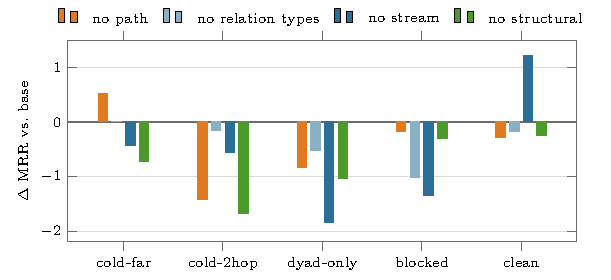
\includegraphics[width=0.82\textwidth]{figures/fig_ablation_strata.pdf}
  \caption{Change of MRR on each stratum of ICEWS18 when a component is removed.}
  \label{fig:ablation-strata}
\end{figure}

\para{Effect on strata.} Fig.~\ref{fig:ablation-strata} breaks the ablation down by stratum. The path intensity matters most on cold-2hop ($-1.42$ MRR when removed), the relation types on the blocked stratum ($-1.02$), the stream encoder on the dyad-only and blocked strata ($-1.85$ and $-1.35$), and the structural intensity on the two cold strata ($-0.72$ and $-1.67$). Each component therefore contributes mainly on the queries it is designed for, which is consistent with the additive combination in Eq.~(\ref{eq:super}).

\para{Attention across candidates.} This block improves MRR by 0.25 on ICEWS18, 0.25 on ICEWS14s (47.18 to 47.43) and 0.09 on GDELT (27.01 to 27.10), and reduces it by 0.20 on YAGO and 0.13 on WIKI. On the yearly datasets a query usually has a single candidate with an ongoing fact, so comparing candidates brings no benefit. The validation MRR leads to the same choice on all five datasets.

\para{Components without clear effect.} The popularity intensity and the candidate context change the results by less than the seed variance on both datasets. Our implementation further contains a prototype term that scores all entities by their similarity to an attention-weighted average of the support entities; removing it changes MRR by $+0.05$ on ICEWS18 and $-0.16$ on YAGO, which is also within the seed variance, so we do not describe it in Sect.~\ref{sec:method}. We report these components as having no clear effect.

% ─────────────────────────────────────────────────────────────────────────
\section{Conclusion}
\label{sec:conclusion}

\para{Summary.} In this paper, we studied which historical evidence a TKG forecasting model should read. A data-only analysis showed that about a quarter of the ICEWS test queries have an answer that interacted with the subject only under other relations, which copy mechanisms cannot handle. We proposed \model{}, which adds four intensities and encodes the typed and timed event stream of each entity pair with a Transformer, extended by a path intensity and attention across candidates. \model{} achieves the best MRR and \hone{} on YAGO, WIKI and GDELT and the best MRR on ICEWS18 among the compared methods. The stratified evaluation and the ablation study confirmed that the dyadic components are effective on event data, where the dyad-only stratum exists.

\para{Limitations and future work.} \model{} is weak on queries whose answer has never interacted with the subject, which make up about one third of the ICEWS test queries, and its \hten{} on ICEWS is lower than that of LogCL and, on ICEWS18, DiffuTKG. In future work, we plan to strengthen the components that score all entities, for example by combining the dyadic evidence with query-specific global graphs or generative decoders, and to extend the stratified evaluation to more baselines under a unified protocol.

\bibliographystyle{splncs04}
\bibliography{references}

\end{document}
